\chapter{Thực Nghiệm và Đánh Giá}
\graphicspath{{Chapter5/Figs/}}

\begin{chapabstract}
Firstly, we introduce the dataset used for training and evaluating in our experiments. We also present the evaluation metrics and explain the reason for choosing those criteria. Then, the experiment results are shown in comparing to other proposed models. Finally, we present how to set up the environments for experiments.
\end{chapabstract}

\section{Tập dữ liệu}
\label{sec:dataset}

Trong thử nghiệm của chúng tôi, chúng tôi sử dụng 600.000 mẫu đào tạo được dán nhãn và 200.000 mẫu thử nghiệm từ tập dữ liệu Endgame Malware BEnchmark for Research (EMBER) \cite{anderson2018ember}.

\begin{figure}[H] 
\centering
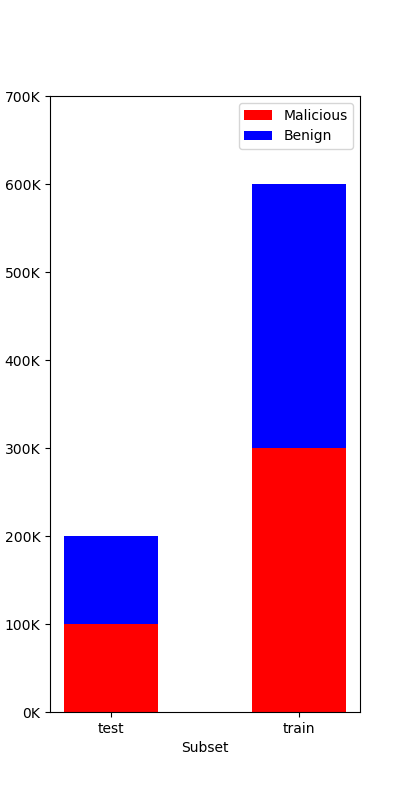
\includegraphics[width=0.5\textwidth]{dataset.png}
\caption{Phân phối mẫu trong tập dữ liệu.}
\label{fig:ember}
\end{figure}
 
Tập dữ liệu EMBER là tập dữ liệu công khai lớn để phát hiện phần mềm độc hại, nó bao gồm các tệp lành tính và có tỷ lệ lý tưởng các tệp độc hại và lành tính cho các tác vụ học máy. Điều này sẽ giải quyết vấn đề chung về độ chính xác dự đoán, cụ thể là vấn đề gây hiểu lầm khi dữ liệu bị mất cân bằng.

\section{Tiêu chí Đánh giá}

Như đã thảo luận trong phần \ref{sec:objectives}, mục tiêu của nghiên cứu là tìm ra phương pháp phát hiện phần mềm độc hại dựa trên học máy hoạt động ở tỷ lệ dương giả thấp trong khi cố gắng đạt được tỷ lệ phát hiện cao.

\subsection{Tỷ lệ Báo động sai}

Sai tích cự (False positive), hoặc báo động sai, xảy ra khi một mô hình sai lầm gán một nhãn độc hại cho một tập tin lành tính. 
Chúng tôi có tập trung làm cho tỷ lệ dương tính giả càng thấp càng tốt, đó là việc không điển hình trong ứng dụng học máy. 
Điều quan trọng là bởi vì ngay cả một báo động giả trong một nghìn tập tin lành tính có thể tạo ra hậu quả nghiêm trọng cho người dùng. 
Vấn đề này là phức tạp bởi thực tế là có rất nhiều tập tin sạch trên thế giới, chúng tiếp tục xuất hiện, và rất khó khăn để thu thập các tập tin này. Chúng tôi đánh giá phương pháp của chúng tôi với hai giá trị báo động giả, cụ thể: ở mức dưới 0,1\% và ở mức dưới 1\%.

\begin{center}
    ${False\ alarm\ rate} =  \cfrac{\sum False\ positive}{\sum Condition\ negative}$
\end{center}

\subsection{Tỷ lệ Phát hiện}

Tỷ lệ phát hiện, (tương đương với recall hoặc true positive rate), đo tỷ lệ các chương trình độc hại được phát hiện trong các tệp phần mềm độc hại được sử dụng để thử nghiệm. Với tỉ lệ cao hơn, ít trường hợp phần mềm độc hại trong thực tế không bị phát hiện. Nói cách khác, tỷ lệ phát hiện cho thấy tiềm năng của các tệp nhị phân độc hại mới sẽ được phát hiện.

\begin{center}
    ${Detection\ rate} =  \cfrac{\sum True\ positive}{\sum Condition\ positive}$
\end{center}

\subsection{Diện tích dưới đường cong ROC}

Như đã giới thiệu trong phần \ref{ssec:auroc}, phần Diện tích dưới đường cong ROC (Area Under the ROC curve, viết tắt là AUROC hoặc AUC) cung cấp thước đo tổng thể về hiệu suất trên tất cả các ngưỡng phân loại có thể có.
AUC là quy mô bất biến và đo lường dự đoán được xếp hạng tốt như thế nào, chứ không phải là giá trị tuyệt đối của chúng.
Bên cạnh đó, AUC là bất biến với ngưỡng phân loại, để nó có thể đo lường chất lượng của các dự đoán không phụ thuộc vào ngưỡng nào được chọn.
Một mô hình có dự đoán là 100\% sai có AUC là 0,0, và có một dự đoán là 100\% đúng có AUC là 1,0.

Hệ thống điểm học thuật điển hình để phân loại độ chính xác của bài kiểm tra phân loại như sau:

\begin{itemize}
\item 0.9 - 1.0 = Excellent
\item 0.8 - 0.9 = Good
\item 0.7 - 0.8 = Fair
\item 0.6 - 0.7 = Poor
\item 0.5 - 0.6 = Fail
\end{itemize}

\section{Kết quả Thực nghiệm}

Phương pháp phát hiện phần mềm độc hại dựa trên GBDT được đề xuất được triển khai với LightGBM framework \cite{ke2017lightgbm}, và các vectơ đặc trưng đầu vào có kích thước 1711. Tất cả các thử nghiệm của chúng tôi đều chạy trên một máy tính ảo hóa có 24 vCPUs và bộ nhớ 32 GB. Sử dụng lập trình song song, mất khoảng 10 phút để vector hóa các tính năng thô và khoảng 5 phút để đào tạo mô hình. Đường cong ROC của mô hình cuối cùng được thể hiện trong hình \ref{fig:roc_curve_with_highlights} và phân phối điểm số cho các mẫu thử được thể hiện trong hình \ref{fig:score_dist}.

\begin{figure}[H]
\centering
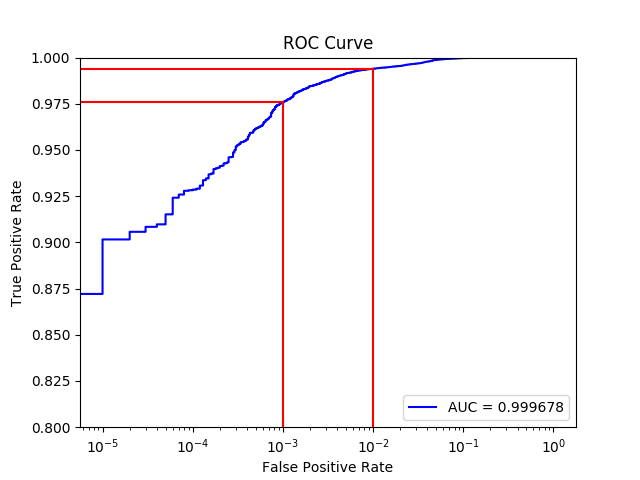
\includegraphics[width=\textwidth]{roc_curve_with_highlights.png}
\caption{The ROC curve of proposed model}
\label{fig:roc_curve_with_highlights}
\end{figure}

\begin{figure}[h] 
\centering
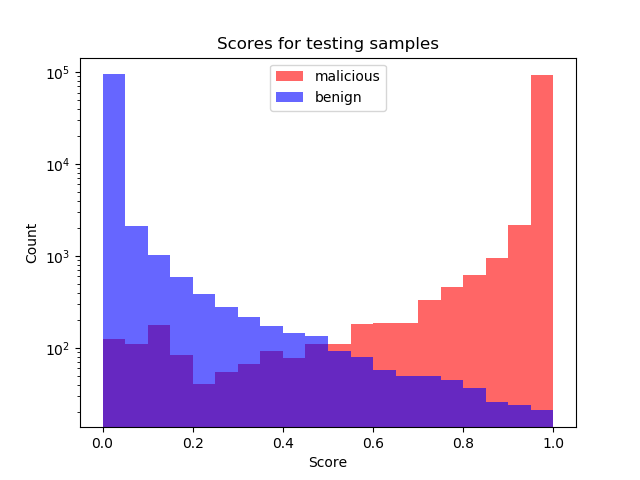
\includegraphics[width=\textwidth]{score_dist.png}
\caption{The distribution of scores for testing samples}
\label{fig:score_dist}
\end{figure}

Diện tích dưới đường cong ROC đạt mức $0.999678$. Với threshold $0.828987$, điểm kết quả của mô hình khi ít hơn $0.1\%$ tỉ lệ báo động sai có tỉ lệ phát hiện $97.5720\%$. Và với mức tỉ lệ báo động sai $1\%$, mô hình đạt tỉ lệ phát hiện $99.3940\%$ với threshold là $0.307897$. 

Mô hình cơ sở của EMBER chỉ có diện tích dưới đường cong ROC là $0.99911$, kết quả với mức $0.1\%$ FPR là $92.99\%$ TPR, và mức $1\%$ FPR, là $98.2\%$ TPR. Mô hình của chúng tôi có hiệu suất tốt hơn do điều chỉnh siêu tham số và cũng mất ít thời gian hơn cho việc đào tạo do giảm số lượng các đặc trưng.Rõ ràng, mô hình có hiệu suất tốt hơn so với mô hình MalConv được đào tạo trên các tệp nhị phân thô \cite{anderson2018ember}, nó có ROC AUC là $0.99821$, tương ứng với $92.2\%$ TPR ở mức báo động sai dưới 0.1\%, và 97.3\% TPR ở mức dưới 1\% FPR. Bảng \ref{table:training-time} và bảng \ref{table:results}hiển thị thời gian đào tạo và kết quả đánh giá của mô hình đề xuất của chúng tôi so với mô hình MalConv và mô hình cơ sở của EMBER.

\begin{table}[H]
\caption{Thời gian đào tạo của mô hình được đề xuất của chúng tôi so với mô hình MalConv và mô hình cơ sở của EMBER}
\centering
\label{table:training-time}
\begin{tabular}{l l l l}
\hline
Model & Input &  Specifications & Training time \\
\hline
MalConv & Raw binaries & \begin{tabular}[c]{@{}l@{}} 2 NVDIA TITAN X \\ (Pascal) GPUs \end{tabular}  & \begin{tabular}[c]{@{}l@{}}10 days\\ (25 hours/epoch)\end{tabular}  \\
EMBER & 2351-value vectors & \begin{tabular}[c]{@{}l@{}} 8 vCPUs \\ (2015 MacBook Pro i7)\end{tabular}  & 20 hours \\ 
Our model & \textbf{1711}-value vectors & \begin{tabular}[c]{@{}l@{}} 24 vCPUs \\ (Google Compute Engine) \end{tabular}  & \textbf{5 minutes }\\ 
\hline 
\end{tabular}
\end{table}

\begin{table}[H]
\caption{Kết quả đánh giá của mô hình được đề xuất của chúng tôi so với mô hình MalConv và mô hình cơ sở của EMBER}
\centering
\label{table:results}
\begin{tabular}{l c c c}
\hline
Model                      & \begin{tabular}[c]{@{}c@{}}False Alarm Rate\\ (FPR)\end{tabular} & \begin{tabular}[c]{@{}c@{}}Detection Rate\\ (TPR)\end{tabular} & \begin{tabular}[c]{@{}c@{}}Area Under\\ the ROC curve (AUC)\end{tabular} \\

\hline
\multirow{2}{*}{MalConv}   & 0.1 \%                 & 92.200 \%            & \multirow{2}{*}{0.998210}                                                 \\
                           & 1.0 \%                 & 97.300 \%            &                                                                           \\
\multirow{2}{*}{EMBER}     & 0.1 \%                 & 92.990 \%            & \multirow{2}{*}{0.999110}                                                 \\
                           & 1.0 \%                 & 98.200 \%            &                                                                           \\
\multirow{2}{*}{Our model} & 0.1 \%                 & 97.572 \%            & \multirow{2}{*}{0.999678}                                                 \\
                           & 1.0 \%                 & 99.394 \%            &                                                                          
\\
\hline 
\end{tabular}
\end{table}

\section{Hướng dẫn cài đặt môi trường} 
\label{sec:research-env}

We mainly use the cross-platform tools in research and development for easily switching between operating systems. We use a Windows 10 Pro virtual machine for static malware analysis, an Ubuntu 16.04 LTS cloud instance for training and testing machine learning models, and use PyCharm Professional as mainly Integrated development environment (IDE).

\subsection{Windows environment for static analysis}

We use a virtual machine to build a background about malware:

\begin{itemize}
\item OS: Microsoft Windows 10 Pro
\item Version: 10.0.17134
\item Architecture: 64-bit
\end{itemize}

With following tools, we can easily gather malware basic information:

\begin{itemize}
 \item \textbf{CFF Explorer}: PE header parser.
 \item \textbf{PE Explorer} (from Heaventools Software): PE inspection tool.
 \item \textbf{BinText} (from McAfee): extract string from a binary.
 \item \textbf{HxD Hex Editor}: support for viewing file in binary format.
\end{itemize}

\subsection{Ubuntu environment for machine learning tasks}

\subsubsection{Google Cloud Platform}

We use an virtual machine for research, that can be deployed with the image from \textit{\href{https://console.cloud.google.com/launcher/details/ubuntu-os-cloud/ubuntu-xenial}{Cloud Launcher - Canonical - Ubuntu Xenial}}. The cloud instance has 24 virtual CPUs, 32 GB for memory, and is located in \verb|asia-southeast1-b| zone, i.e., Jurong West, Singapore.

After deployment, we add two optional firewall rules (\textit{\href{https://console.cloud.google.com/networking/firewalls/add}{VPC network - Firewall rules - Create a firewall rule}}), which allows all in and out connections for the virtual machine, to use Python Interactive Console features in PyCharm IDE.

\subsubsection{Anaconda}

We choose Anaconda, a free and open source distribution of the Python, to manage package and deploy. The content of \verb|environment.yml| used to deploy is shown below. 

\begin{lstlisting}
name: lab
channels:
  - conda-forge
dependencies:
  - python==3.6
  - matplotlib
  - numpy
  - scikit-learn
  - pip:
    - lief
    - git+https://github.com/onnx/onnxmltools
    - lightgbm
\end{lstlisting}

The environment is created with \textbf{Python 3.6} and packages for machine learning:

\begin{itemize}
\item \textbf{NumPy}: the fundamental package for scientific computing with Python.
\item \textbf{Matplotlib}: a Python 2D plotting library.
\item \textbf{Scikit-learn}: a machine learning library.
\item \textbf{Lief}: library to instrument executable formats.
\item \textbf{LightGBM}: a gradient boosting framework based on decision tree algorithms.
\item \textbf{ONNXMLTools}: a tool to convert models to ONNX format.
\end{itemize}

\subsection{PyCharm Professional IDE}

JetBrains provides \textit{\href{https://www.jetbrains.com/student/}{free individual licenses for students}} to use PyCharm Professional IDE. This is the powerful Python IDE, which gives us remote development capabilities and supports many scientific tools (e.g., Anaconda, Matplotlib and NumPy).

Following the guide \textit{\href{https://www.jetbrains.com/help/pycharm/configuring-remote-interpreters-via-ssh.html}{Configuring Remote Interpreters via SSH}} published by JetBrains, we can run, debug remotely from a cloud instance, which gives a great performance and is easy to scale.
